\documentclass{article}
\usepackage[utf8]{inputenc}
\usepackage[margin=1in]{geometry}
\usepackage{amsmath}
\usepackage{graphicx}
\setlength{\parindent}{0em}
\setlength{\parskip}{0.5em}


\title{CTA200 2021 Assignment 2}
\author{Alicia Savelli}
\date{May 8, 2021}

\begin{document}

\maketitle

\section{Question 1}

\subsection{Methods}
For this problem, the derivative of $f(x)=\sin(x)$ was approximated using two methods.  The first method was taking the derivative using first principles about about a point $x_0$ with infinitesimal step $h$ as $h \xrightarrow[]{} 0$,

\begin{equation}
    d_x f|_{x_0} \approx \frac{f_{x_0 + h} - f_{x_0}}{h}.
    \label{eq:m1}
\end{equation}

A better approximation can be found when $h$ is instead finite using
\begin{equation}
    d_x f|_{x_0} \approx \frac{f_{x_0 + h} - f_{x_0 - h}}{2h}.
    \label{eq:m2}
\end{equation}

The derivative of $f(x)=\sin(x)$ for $x_0 = 0.1$ was taken using both methods for increasingly small values of $h$.  The error of the numerical derivative was compared to the analytical derivative was plotted as a function of $h$ on a double log plot for each method, as seen in Figure~\ref{fig:q1}.  

\subsection{Analysis}
The values for the approximation of $\frac{d}{dx} \sin(x) |_{x_0}$ for increasingly small values of $h$ are shown in Table~\ref{tab:h}.

\begin{table}[h]
\caption{Approximation of $\frac{d}{dx} \sin(x) |_{x_0}$ for $x_0=0.1$}
\label{tab:h}
\vspace{0.15in}
\begin{center}
\begin{tabular}{|c|c|c|}
\hline
$h$ & Method 1 & Method 2 \\
\hline
1e-1 & 0.9883591414823306 & 0.9933466539753061 \\
1e-3 & 0.994954082739849 & 0.995003999444008 \\
1e-9 & 0.9950041623962845 & 0.9950041623962845 \\
1e-15 & 0.9992007221626408 & 0.9922618282587335 \\
\hline
\end{tabular}
\end{center}  
\end{table}

\begin{figure}[!h]
  \centering{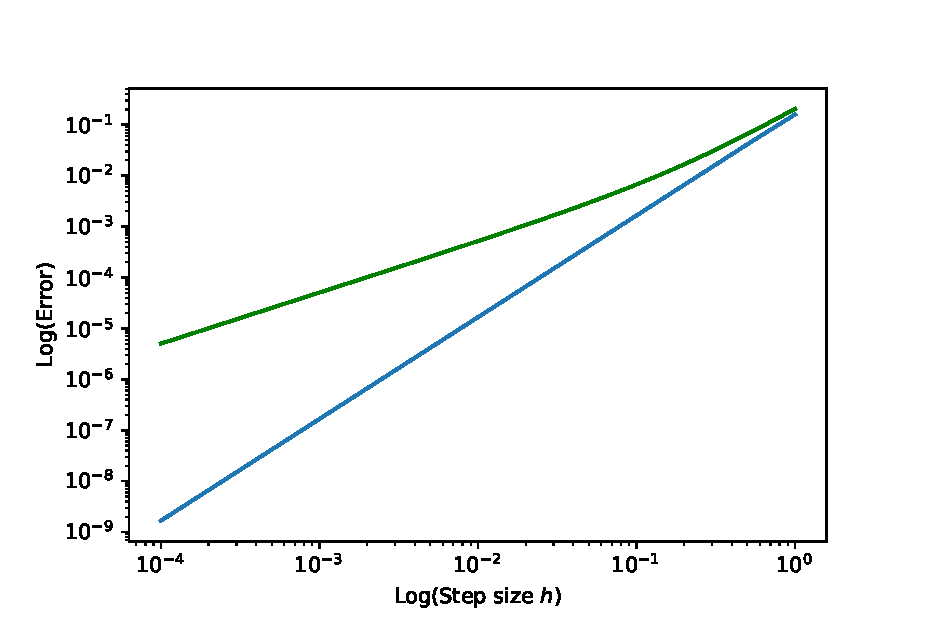
\includegraphics[width=0.8\textwidth]{q1.eps}
    \caption{Loglog plot of error in numerical approximation of the derivative of $f(x)=\sin(x)$ using Method 1 (green) and Method 2 (blue).}}
    \label{fig:q1}
\end{figure}

As can be seen from the table, both methods give similar results for larger values of $h$, but as $h$ decreases these values diverge from one another.  From the plot of the error in Figure~\ref{fig:q1}, we can see that Method 2 gives a better approximation of the true derivative of $f(x)=\sin(x)$ since its error goes to zero much quicker than that for Method 1.  The steeper slope of the plot for Method 2 indicates that the approximation of the derivative about $x_0$ converges more quickly than the approximation using Method 1.

\section{Question 2}

\subsection{Methods}
The equation 

\begin{equation}
    z_{i+1}=z_i^2 + c
    \label{eq:z}
\end{equation}

where $c=x+iy$ for $-2<x<2$ and $-2<y<2$, and $z_0=0$, will converge for some points in the complex plane $c$ and diverge for others.  2000 values for both $x$ and $y$ were generated and then iterated through Equation~\ref{eq:z} 255 times.  If $|z^2|$ remained bounded (i.e. $|z^2|$ $<$ a large number) for all iterations, $z$ was said to diverge at that point.  Otherwise, $z$ was said to converge. The data for each iteration at each point was stored in arrays and plotted both as a Boolean function of divergence (see Figure~\ref{fig:q2a}) and as a gradient indicating the iteration at which $z$ diverges at a given point $c$ (see Figure~\ref{fig:q2b}).

\subsection{Analysis}
The plots of the results of the Boolean function of divergence and the gradient indicating the iteration at which $z$ diverges at a given point $c$ can be seen in Figures~\ref{fig:q2a} and~\ref{fig:q2b}, respectively.  The resolution of the images is sharper for a larger set of values of $x$ and $y$, however adding these iterations dramatically increases the computation time.  The figures show the Mandelbrot set.

\begin{figure}[!h]
  \centering{
\includegraphics[width=0.8\textwidth]{q2a.eps}
    \caption{Plot of $z_{i+1}=z_i^2+c$, colouring is Boolean-based on whether a given point $c = x + iy$ converges (white) or diverges (black) after 255 iterations.}}
    \label{fig:q2a}
\end{figure}

\begin{figure}[!h]
  \centering{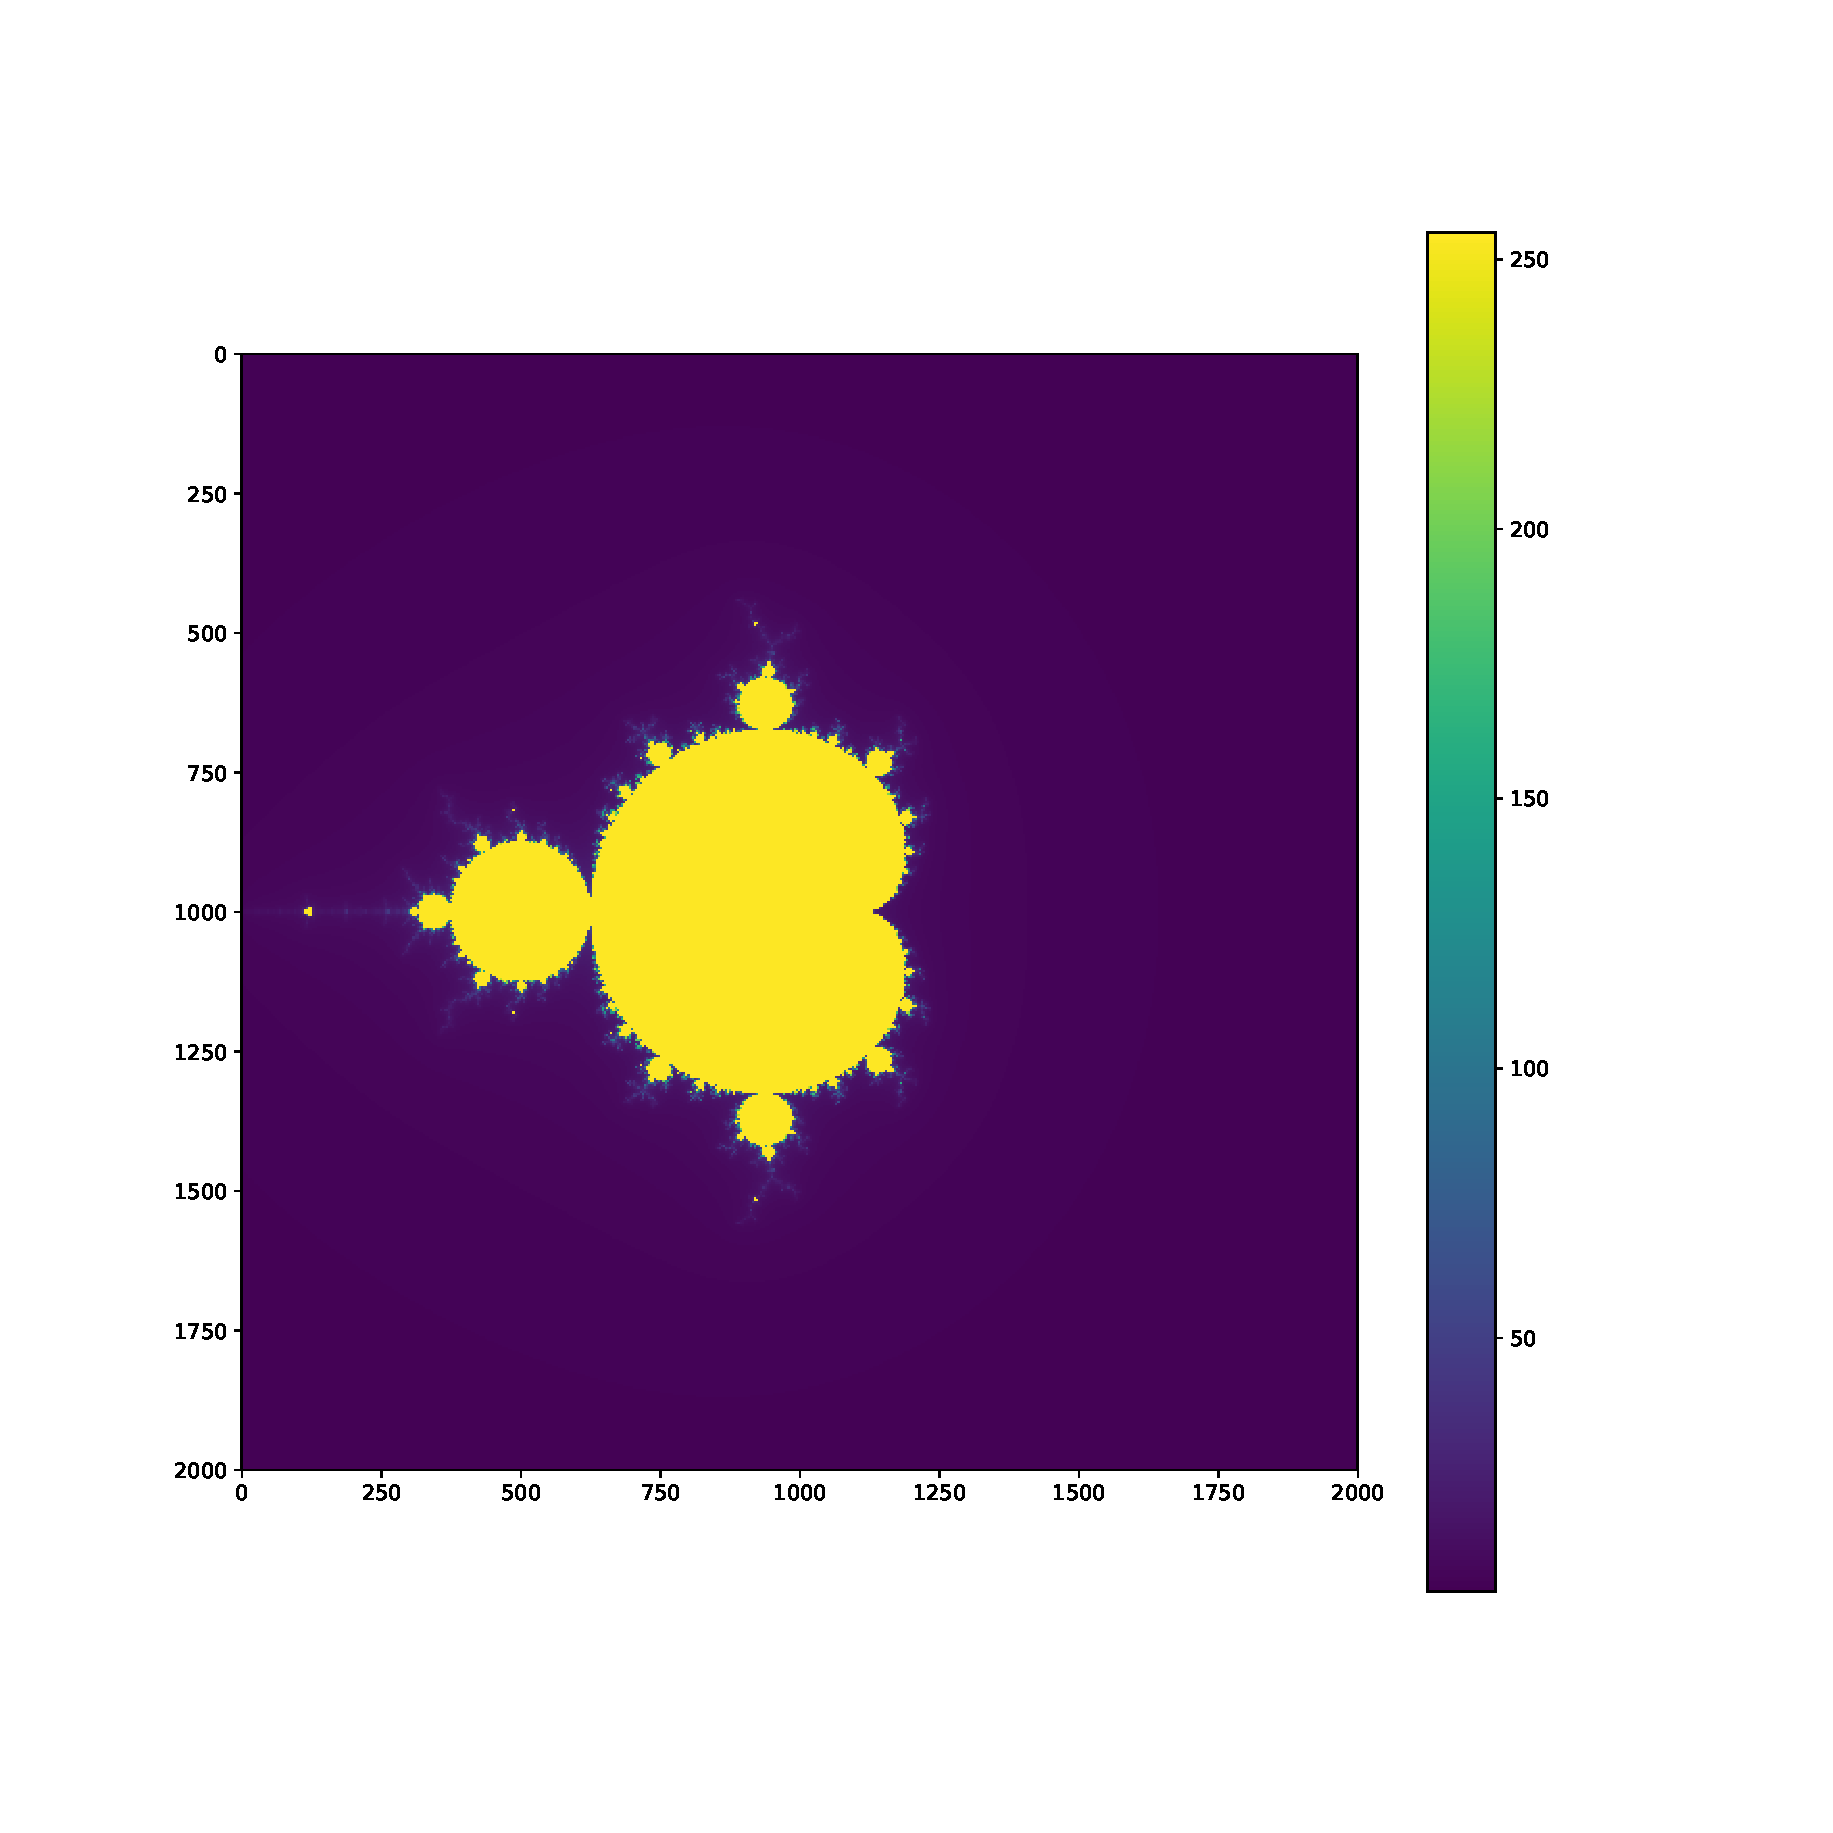
\includegraphics[width=0.8\textwidth]{q2b.eps}
    \caption{Plot of $z_{i+1}=z_i^2+c$, colourmap is based on the iteration at which the given point $c = x + iy$ diverges - colouring is yellow if $c$ converges after 255 iterations.}}
    \label{fig:q2b}
\end{figure}

\section{Question 3}

\subsection{Methods}
In this problem, the SIR model for the spread of infectious diseases was analyzed using a system of 3 first order ODE's:

\begin{eqnarray}
    \frac{dS}{dt} & = & -\frac{\beta S I}{N}, \\
    \label{eq:S}
    \frac{dI}{dt} & = & \frac{\beta S I}{N} - \gamma I, \\
    \label{eq:I}
    \frac{dR}{dt} & = & \gamma I
    \label{eq:R}
\end{eqnarray}

representing the individuals in a fixed population size $N=1000$ who are susceptible to the disease but not yet infected, infected, and recovered from the disease with immunity (sometimes called ``removed"), respectively.  The parameter $\beta$ describes the rate of infection of exposed individuals, and the parameter $\gamma$ describes the inverse of the average length of infection. 

The system of equations was solved using the ODE integrator {\tt dopri5} imported from the {\tt Scipy} module and the initial conditions $S(0)=999$, $I(0)=1$, and $R(0)=0$.  Various combinations of values for the parameters of $\beta$ and $\gamma$ were used to solve the equations.  The solutions can be seen in the four plots of Figure~\ref{fig:q3}.

\subsection{Analysis}
Four combinations of values for $\beta$ and $\gamma$ were chosen to demonstrate drastic differences in the results.  A high probability of infection ($\beta=0.9)$ and a long recovery period ($\gamma=10$) days are simulated in the top left plot.  This combination shows a virus that infects over half of the population but would be virtually wiped out after 50 days from the initial infection.  The top right plot shows a simulation of an infection with a moderate rate of infection ($\beta=0.7$) and a short period of infection ($\gamma \approx 1.5$ days), resulting in a disease that also takes 50 days to be wiped out from the community but is only contracted by about 1/10$^{\rm{th}}$ of the population.  A model with a moderate infection rate ($\beta=0.5$) and a very short recovery period ($\gamma \approx 1$ day) is shown in the bottom left plot.  This simulation shows a disease that infects nearly none of the overall population and does not seem to have a significant impact on the community.  The plot in the bottom right shows a simulation with a low infection rate ($\beta = 0.2$) and a long recovery period ($\gamma = 100$ days).  This model shows a virus that infects almost every individual in the population, and takes a very long time to be wiped from the community.  

\begin{figure}[!h]
  \centering{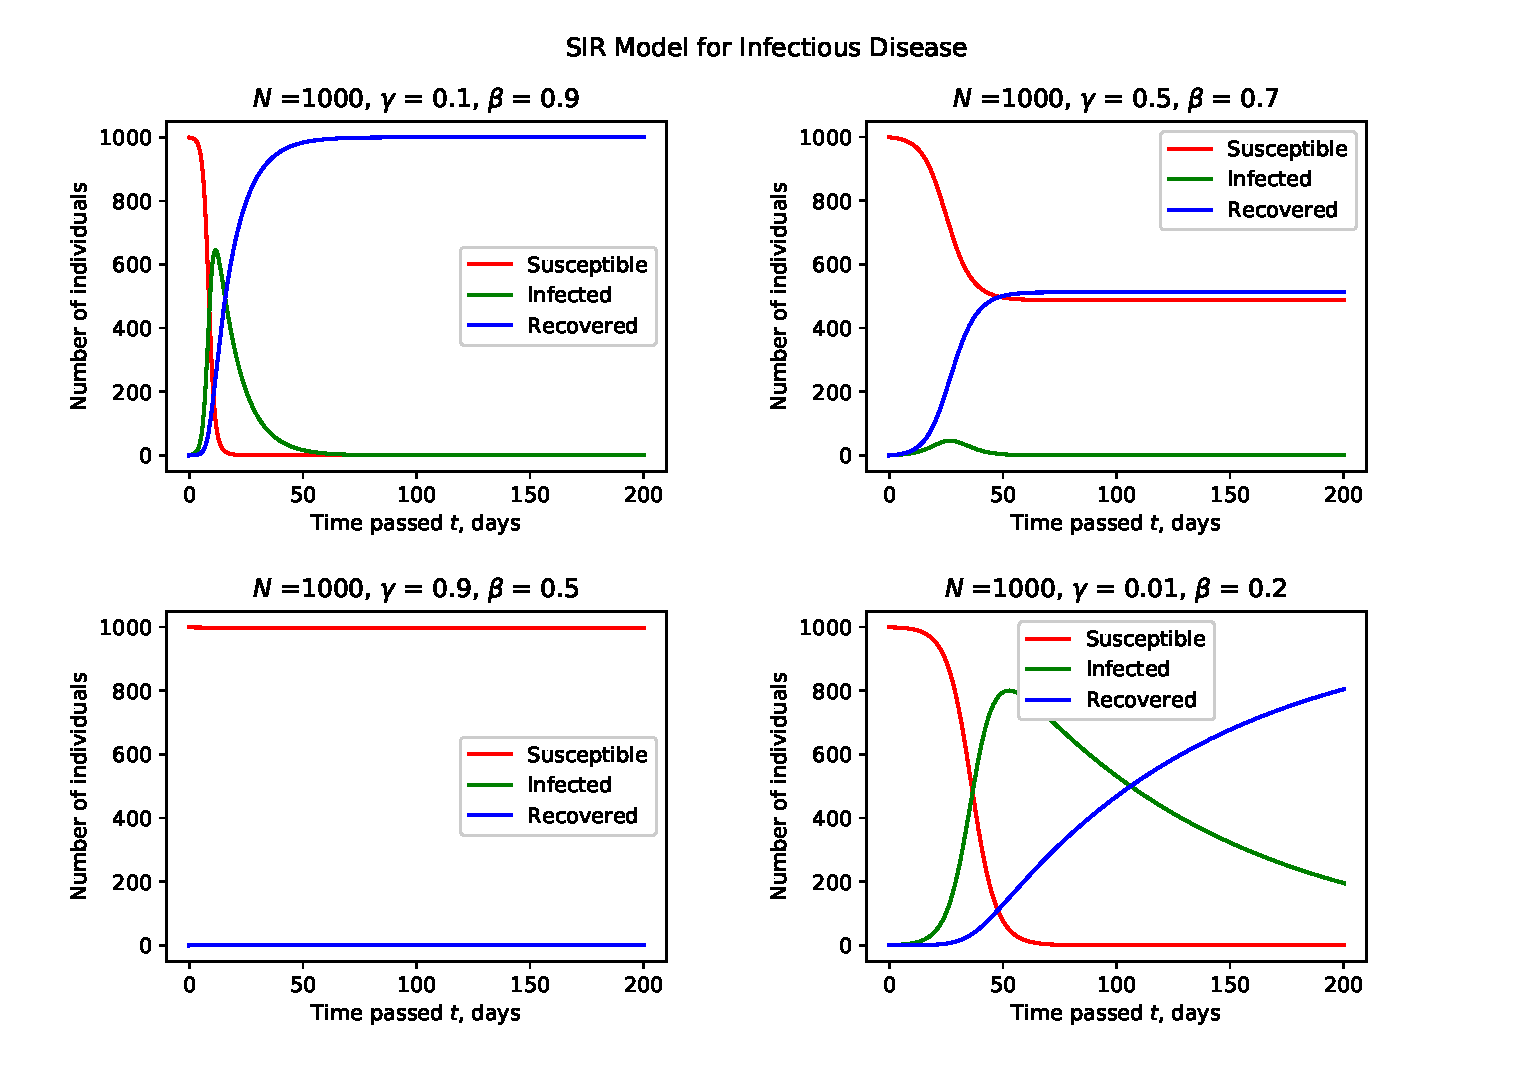
\includegraphics[width=1\textwidth]{q3.eps}
    \caption{Plots of SIR model for infectious diseases for various parameters recovery rate, $\gamma$, and infection rate, $\beta$.}}
    \label{fig:q3}
\end{figure}

\end{document}

